%\documentclass[gray]{jmlr} % test grayscale version
%\documentclass[tablecaption=bottom]{jmlr}% journal article
\documentclass[pmlr,twocolumn,10pt]{jmlr} % W&CP article

% The following packages will be automatically loaded:
% amsmath, amssymb, natbib, graphicx, url, algorithm2e

%\usepackage{rotating}% for sideways figures and tables
%\usepackage{longtable}% for long tables

% The booktabs package is used by this sample document
% (it provides \toprule, \midrule and \bottomrule).
% Remove the next line if you don't require it.

\usepackage{booktabs}
% The siunitx package is used by this sample document
% to align numbers in a column by their decimal point.
% Remove the next line if you don't require it.
%\usepackage[load-configurations=version-1]{siunitx} % newer version 
\usepackage{siunitx}

\usepackage{csquotes} %fancy quotes
\usepackage{braket} %bra-ket formalism
\usepackage{graphicx,caption} %caption regulation


% The following is to recognise equal contribution for authorship
\newcommand{\equal}[1]{{\hypersetup{linkcolor=black}\thanks{#1}}}

% Define an unnumbered theorem just for this sample document for
% illustrative purposes:
\theorembodyfont{\upshape}
\theoremheaderfont{\scshape}
\theorempostheader{:}
\theoremsep{\newline}
\newtheorem*{note}{Note}

% change the arguments, as appropriate, in the following:
\jmlrvolume{}
\jmlryear{2023}
\jmlrsubmitted{}
\jmlrpublished{}
\jmlrworkshop{Controversies in Game Theory} % W&CP title

% The optional argument of \title is used in the header
\title[Quantum Beauty Contest]{Quantum Beauty Contest}

% Anything in the title that should appear in the main title but 
% not in the article's header or the volume's table of
% contents should be placed inside \titletag{}

%\title{Title of the Article\titletag{\thanks{Some footnote}}}


% Use \Name{Author Name} to specify the name.
% If the surname contains spaces, enclose the surname
% in braces, e.g. \Name{John {Smith Jones}} similarly
% if the name has a "von" part, e.g \Name{Jane {de Winter}}.
% If the first letter in the forenames is a diacritic
% enclose the diacritic in braces, e.g. \Name{{\'E}louise Smith}

% \thanks must come after \Name{...} not inside the argument for
% example \Name{John Smith}\nametag{\thanks{A note}} NOT \Name{John
% Smith\thanks{A note}}

% Anything in the name that should appear in the title but not in the 
% article's header or footer or in the volume's
% table of contents should be placed inside \nametag{}

% Two authors with the same address
% \author{%
%  \Name{Author Name1\nametag{\thanks{A note}}} \Email{abc@sample.com}\and
%  \Name{Author Name2} \Email{xyz@sample.com}\\
%  \addr Address
% }

% Three or more authors with the same address:
% \author{%
%  \Name{Author Name1} \Email{an1@sample.com}\\
%  \Name{Author Name2} \Email{an2@sample.com}\\
%  \Name{Author Name3} \Email{an3@sample.com}\\
%  \Name{Author Name4} \Email{an4@sample.com}\\
%  \Name{Author Name5} \Email{an5@sample.com}\\
%  \Name{Author Name6} \Email{an6@sample.com}\\
%  \Name{Author Name7} \Email{an7@sample.com}\\
%  \Name{Author Name8} \Email{an8@sample.com}\\
%  \Name{Author Name9} \Email{an9@sample.com}\\
%  \Name{Author Name10} \Email{an10@sample.com}\\
%  \Name{Author Name11} \Email{an11@sample.com}\\
%  \Name{Author Name12} \Email{an12@sample.com}\\
%  \Name{Author Name13} \Email{an13@sample.com}\\
%  \Name{Author Name14} \Email{an14@sample.com}\\
%  \addr Address
% }

% Authors with different addresses and equal first authors:
\author{%
\Name{Philipp Pestlin}\Email{ppestlin@ethz.ch}\\
\addr D-CHAB, ETH Zürich
\AND
% footnotemark[1] is to refer to the \equal footnote
\Name{Tommaso Antonelli} \Email{tantonelli@ethz.ch}\\
\addr D-PHYS, ETH Zürich
\AND
\Name{Yoel Zimmermann} \Email{yzimmermann@ethz.ch}\\
\addr D-CHAB, ETH Zürich
}

\begin{document}
\maketitle
% GITHUB REPO: https://github.com/yzimmermann/QBC

\begin{abstract}
\vspace{-0.6cm}\\
We introduce a quantum version of the Keynesian Beauty Contest game, based on the superposition of the players' guesses. We further analyze the strategy space of this game by means of an evolutionary algorithm in analogy to level k thinking. Through minor modifications to the game dynamics, we assess various approaches and observe diverse equilibrium outcomes. We identify a particular version of the game that shows a preference for pure states above the state $\ket{0}$ corresponding to the classical Nash equilibrium, dependent on specific parameters.
In a projective approach we find a phase transition from an initially unordered to an ordered phase. The time of the phase transition is found to be strongly dependent on the random seed. This approach favors almost pure $\ket{0}$ states at equilibrium. We also show chaotic games where our algorithm can not find dominant strategies as well as an approach that converges but also shows slight deviation from the classical Nash equilibrium as the expectated value.
\end{abstract}
\section{Introduction}
Historically, the Keynesian Beauty Contest is a game that describes the interaction of rational agents in a context where they are asked to choose the most attractive person among a group of people. The players who picked the most popular face are then rewarded with a prize.\\

The catch of this game is that the player should not really pick the most attractive person according to their personal opinion, but rather be aware of the opinions of the other agents in order to formulate a decision. This line of thought can be carried recursively, since the player can then formulate their decision based on their expected opinion of the other players' public perception of beauty, and so on.\\

In the words of John Maynard Keynes himself:
\begin{displayquote}
``...it is not a case of choosing those [faces] that, to the best of one's judgment, are really the prettiest, nor even those that average opinion genuinely thinks the prettiest. We have reached the third degree where we devote our intelligences to anticipating what average opinion expects the average opinion to be. And there are some, I believe, who practice the fourth, fifth and higher degrees." \citep{Keynes_1936}
\end{displayquote}
Also, as Keynes remarks in this work, the Beauty Contest has strong parallels with the behavior of professional investors in financial markets, in the sense that investors try to be one step ahead of the average investor, who is seen as an ignorant agent likely to be present in the market \citep{Duffy1997beauty}.\\

All the features that characterize this historical version of the Beauty Contest can be elegantly put in a mathematical framework that formalizes the setup. In the following section, we will first discuss this classical version of the game, which is a standard introductory example in Game Theory courses. We will then devote our attention to the formulation, computational implementation, and analysis of a quantum version of the game.\\


\section{Theory}
\subsection{Classical Beauty Contest}

The classical Beauty Contest game\footnote{Also widely referred to as Guess 2/3 of the average \citep{ledoux1981concours}, p-contest \citep{kennerberg2019convergence}, and p-guessing game \citep{vie2021evolutionary}} can be mathematically formulated as a set of $N$ players, each of them choosing an integer number in some interval, often from 0 to 100. The mean value $\bar{n}$ of these $N$ numbers is then calculated, and given a certain positive constant $p$ (generally known by all players before the game), the winning number of the contest is given by $w=p\,\bar{n}$ (rounded to the closest integer in the range). The value $p$, commonly taken to be $1/2$ or $2/3$, determines a shift of the winning number from the mean guess and therefore represents the motivation for a certain level of recursive reasoning in the player's choice, analogous to the original Beauty Contest formulation.

As an example of a contractive Beauty Contest with a factor $p=2/3$, the first histogram in Fig. \ref{fig:1} shows that a common strategy is to choose numbers close to the value $50\cdot p^k$ for some positive integer $k$ (i.e., 33, 22, ...). This indicates the different levels of recursion in the decision process, where one starts with the assumption that everybody will play a random number, producing most likely $\bar{n}=50$, and hence playing a value $50\cdot p\simeq 33$. The next step is to think that everybody will most likely play $33$, hence the guess is $33\cdot p=22$. This line of reasoning is called the $k$-level thinking model, where a player tries to outsmart the other players by playing one level ahead of them. This model predicts that agents will learn about their respective environment in successively played games and seems to fairly accurately predict the popular guesses, at least for small values of $k$.

Another popular guess in this iteration of the Beauty Contest seems to be 0, which is basically the limit of this $k$-level model when $k\to\infty$. In fact, the scenario where every player guesses 0 is the unique Nash equilibrium for the Beauty Contest game (given $0<p<1$) \citep{kennerberg2019convergence}. However, in this case, the assumption of perfect rationality of the other players is a strong one, and it is very naive to imagine that all people will take this $k$-level model to the extreme consequences, thus practically invalidating the strategy of playing 0.

As expected, in this first iteration of the Beauty Contest with $p=2/3$, the winning number is not $w=0$, but rather $w=20$. If the same game is repeated with the same group of $N$ people, the consequence is visible: people seem to adapt to the game environment and play on average much lower numbers, as seen in the last two histograms in Fig. \ref{fig:1}.

It's now time to go quantum!

\begin{figure}[h]
    \centering
    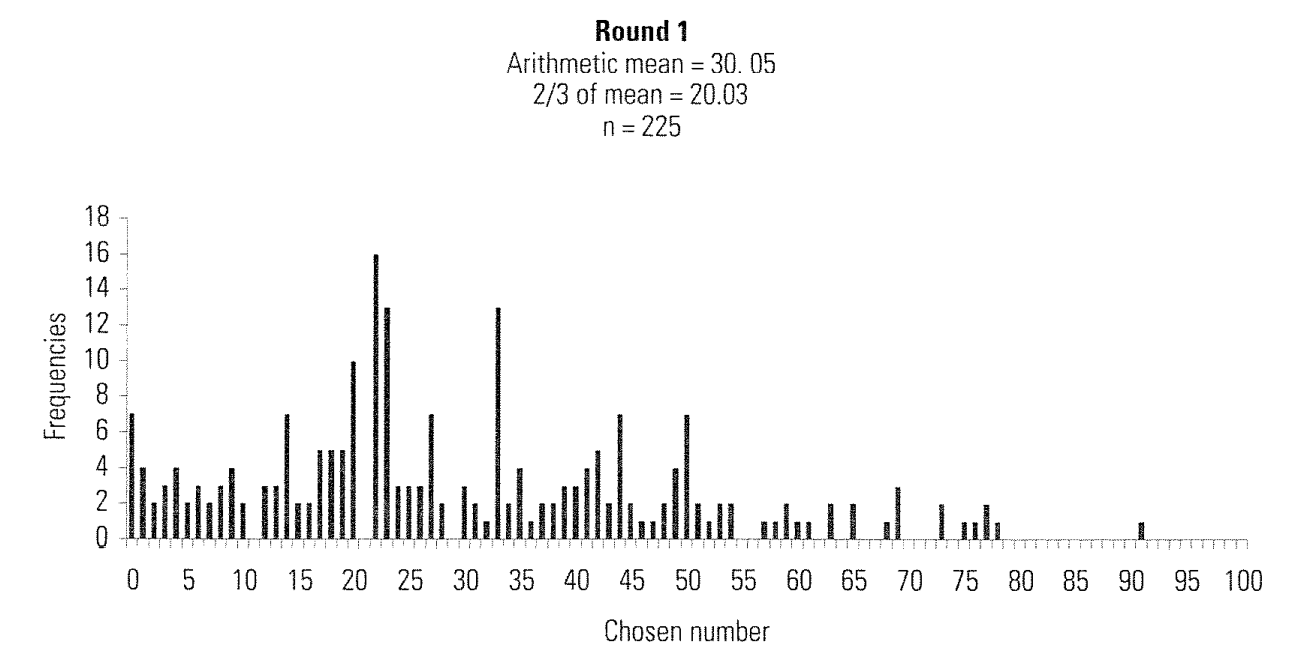
\includegraphics[width=0.45\textwidth]{chil-template-2023/images/round1_classical.png}\vspace{0.5cm}
    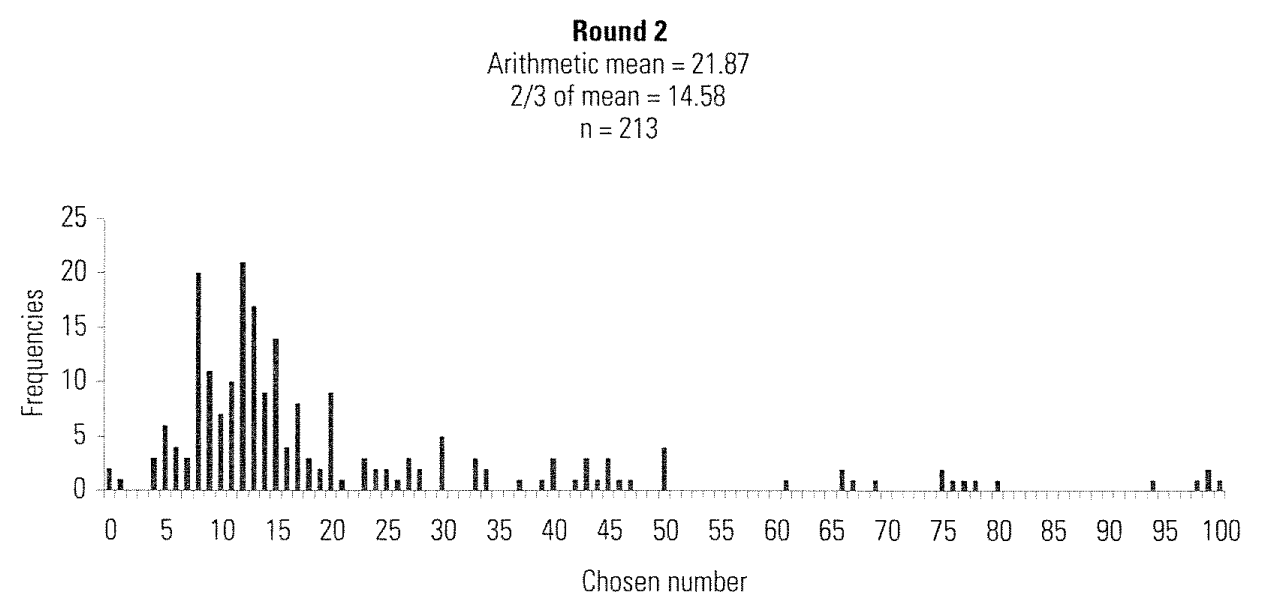
\includegraphics[width=0.45\textwidth]{chil-template-2023/images/round2_classical.png}\vspace{0.5cm}
    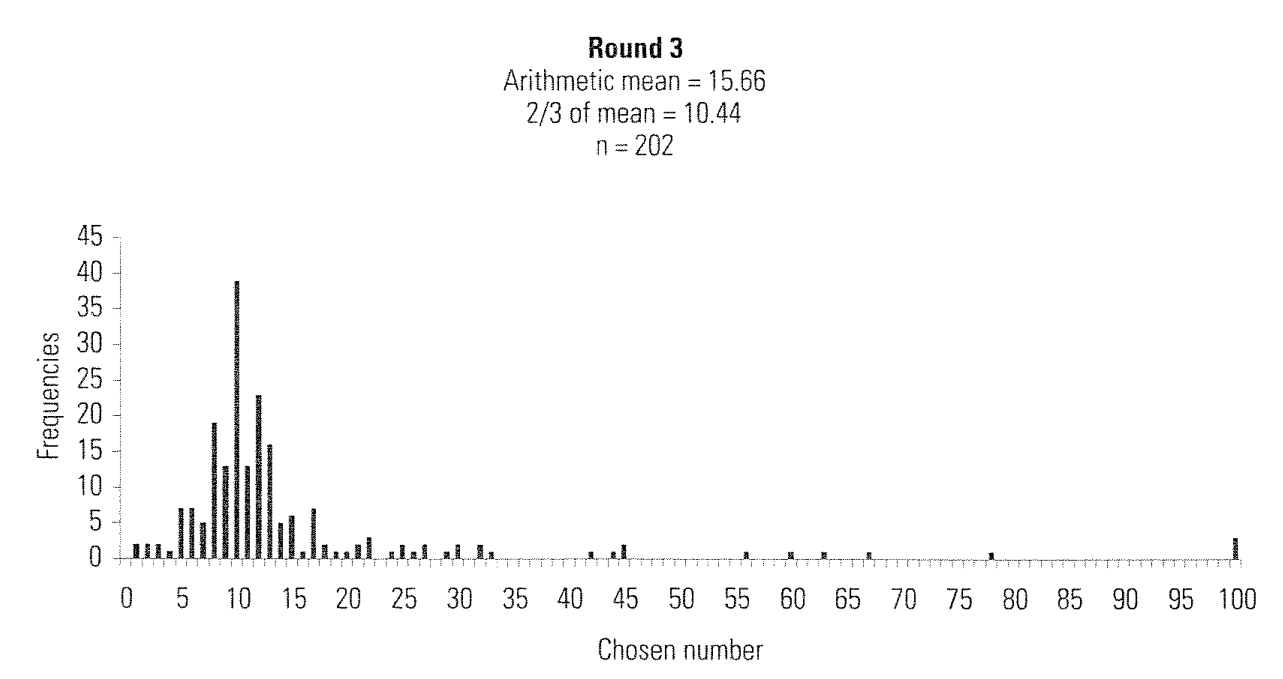
\includegraphics[width=0.45\textwidth]{chil-template-2023/images/round3_classical.png}
    \caption{From top to bottom: the first three rounds of the classical Beauty Contest results, with a value of $p=2/3$ \citep{diekmann2009classical}.}
    \label{fig:1}
\end{figure}

\subsection{Quantum Beauty Contest}

The game we are considering again involves $N$ players, each of whom will formulate a guess. In this scenario, however, the guess is formulated in terms of quantum states. For this, we construct a $(M+1)$-dimensional Hilbert space $\mathcal{H}_M$, where, for concreteness, we will choose $M=100$. This space is spanned by the following base kets, in standard Dirac notation:
\begin{equation}
  \label{eq:basis}
  \Bigl\{\ket{0},\ \ket{1},\ \ket{2},\,...\,\ket{100}\Bigr\}
\end{equation}

which are the eigenstates of a number operator $\hat{N}$ with the explicit form
\begin{equation}
    \hat{N} = \sum_{n=0}^{100} n \ket{n}\bra{n}
\end{equation}

from which we can immediately see the defining property
\begin{equation}
    \label{eq:number_operator}
    \hat{N}\ket{n} = n \ket{n}.
\end{equation}

Furthermore, the basis is generally chosen to be normalized:
\begin{equation}
    \label{eq:normalization}
    \braket{n|m} = \delta_{nm}
\end{equation}

where $\delta_{nm}$ is the Kronecker delta.

In a certain sense, the base kets represent the guesses a player can make in the classical game. Now, in this variation of the game, each player is asked to give a guess in the form of a normalized ket:
\begin{equation}
  \ket{\psi_i}\in\mathcal{H}_M \quad \text{for}\quad  i\in\{1,2,\,...\,N\},
\end{equation}

i.e.,
\begin{equation}
    \ket{\psi_i} = \sum_{n=0}^{100} c_n^{(i)} \ket{n}\quad \text{and}\quad \sum_{n=0}^{100} \, |c_n^{(i)}|^2 = 1\quad \forall i.
\end{equation}

Then the following ket state is constructed:
\begin{equation}
\label{eq:game_ket}
  \ket{\psi}=\mathcal{N}\,\sum_{i=1}^{N}\ket{\psi_i}
\end{equation}

where $\mathcal{N}$ is some normalization constant.

The next step is to collapse our state $\ket{\psi}$ into the basis given in Eq. \ref{eq:basis}, that is to say, we perform a measurement of $\hat{N}$ on $\ket{\psi}$.

We will therefore obtain the state ket
\begin{equation}
  \ket{n},\quad \text{with }n\in\{0,1,\,...\,100\}
\end{equation}

with a probability
\begin{equation}
  P_n=|\braket{n|\psi}|^2.
\end{equation}

The winning number is then determined as usual:
\begin{equation}
  w=\text{round}(p\cdot n)
\end{equation}

for some positive $p$. With this number, we can single out the basis ket $\ket{w}$ and determine the winner(s) of the Quantum Beauty Contest by assigning a payoff to each player using the following formula:
\begin{equation}
  \phi_i=|\braket{w|\psi_i}|^2
\end{equation}

which is basically a simple measure for determining how much of the winning outcome was contained in the player's initial guess.

From a theoretical point of view, the Quantum Beauty Contest we propose does not reduce to its classical analogue for any choice of the players' strategies. This is due to two independent features of the quantum version of the game.

Firstly, the winning number $w$ is produced through a measurement procedure of the state $\ket{\psi}$, hence there is a component of randomness in this game that is not present in the classical version.

Secondly, even if one repeated the measurement of the same state $\ket{\psi}$ over and over again, thus effectively extracting the mean value of the operator $\hat{N}$ (which will be in fact done in some later computational implementations of the game), in general, there is no strategy of the players that can simulate the classical analogue of the game. This is because the way we decided to construct the state $\ket{\psi}$ is through the sum with equal weights of the guesses $\ket{\psi_i}$. In this game, the only strategy that resembles a classical game is for every player to play a ket in the basis of Eq. \ref{eq:basis}:
\begin{equation}
  \ket{\psi_i}=\ket{n},\quad \text{for some }n\in\{0,1,\,...\,100\}
\end{equation}

In this way, though, if two players decide to play the same number, i.e., $\ket{\psi_i}=\ket{\psi_j}=\ket{n}$ with $i\neq j$, then the probability amplitudes in the state $\ket{\psi}$ for the basis state $\ket{n}$ add up, while the actual probability of extracting the number $n$ goes as the amplitude squared. This is in contrast with the classical game, where every instance of a guess $n$ simply adds up, and the mean is calculated afterwards without squaring the columns of the histogram.

Anyway, apart from these differences, the spirit of the game remains the same, but in this case, the strategy space is much richer than the classical counterpart.


\section{Computation}
The strategies of the Quantum Beauty Contest reside in a high-dimensional Hilbert space. To effectively explore and optimize these strategies, an evolutionary algorithm is employed. The algorithm utilizes reproduction and mutation, enabling effective sampling of the strategy space to find optimal strategies. A similar algorithm has recently been used to computationally study the prisoner's dilemma \citep{vie2021evolutionary}.\\

\subsection{Reproduction}

Let $\ket{{\text{S}_1}}$ and $\ket{{\text{S}_2}}$ represent the quantum states of two parent strategies. The reproduction operator $R: \mathcal{H} \times \mathcal{H} \rightarrow \mathcal{H}$ combines these states to generate a new strategy for the offspring:
\begin{equation}
\ket{\text{S}_{\text{offspring}}} = {R}\left(\ket{\text{S}_1}, \ket{{\text{S}_2}}\right) = \mathcal{N}(\ket{\text{S}_1} + \ket{{\text{S}_2}})
\end{equation}

This process ensures that the offspring inherits characteristics from both parents while exploring new regions of the strategy space.\\

\subsection{Mutation}

The mutation operator introduces variation by perturbing individual strategies after reproduction.\\

Let's denote the mutation operator as $M(\ket{S}, \pi, \sigma)$, where $\ket{S}$ is some strategy, $\pi$ is the mutation rate, and $\sigma$ is the mutation strength. The mutation operator can be defined as follows:
\begin{align}
&M(\ket{S}, \pi, \sigma) = \ket{S'}\
&\ket{S'}_i = \left{
\begin{array}{ll}
\ket{S}_i + \delta & \text{with probability } \pi \
\ket{S}_i & \text{with probability } 1 - \pi
\end{array}
\right.
\end{align}

where $\ket{S'}$ represents the mutated strategy, and $\delta$ is a random perturbation drawn from a uniform distribution $\mathcal{U}(\left[-\sigma, \sigma\right])$. If a mutation event occurs (with probability $\pi$), the corresponding component of the strategy is perturbed by adding a random value from $\delta$. Therefore, a higher mutation rate leads to more frequent mutations and greater exploration of the strategy space, while a lower mutation rate promotes exploitation of existing elite strategies.\\

On the other hand, a larger mutation strength results in larger deviations from the original strategy, allowing for more significant exploration of the strategy space. Conversely, a smaller mutation strength limits the extent of perturbations, promoting finer adjustments to the strategies.\\

\subsection{Algorithm}

Here is a quick overview of the algorithm employed:
\begin{enumerate}
\item \textbf{Initialize:} For every player $i$, draw random strategy ket $\ket{S_i} \sim \mathcal{U}_{101}(\left[-1, 1\right]^{101})$ with $\braket{S_i|S_i}=1$.
\item \textbf{Simulate Game:}
\subitem \hspace{-0.7cm}a. Draw $\ket{n}$ from $|\braket{\psi|\psi}|^2$ as defined in Eq. \ref{eq:game_ket} and determine winner ket $\ket{w}$.
\subitem \hspace{-0.7cm}b. Determine the fitness of $\ket{\text{S}_i}$ with respect to $\ket{w}$ for every strategy.
\item \textbf{Reproduction Cycle}
\subitem \hspace{-0.7cm}a. Extract a fixed number of elite strategies into the new game.
\subitem \hspace{-0.7cm}b. Select parent strategies $\ket{\text{S}_i}$ and $\ket{\text{S}_j}$ ($i \neq j$) and form a new strategy $M(R(\ket{\text{S}_i}, \ket{\text{S}_j}), \pi, \sigma)$.
\subitem \hspace{-0.7cm}c. Repeat b. until every player has a strategy.
\item \textbf{Iterate:} Jump to step 2. until convergence or a fixed number of iterations is reached.
\end{enumerate}

For the specific implementation of the game, we can make different choices for how we determine $\ket{w}$ as well as the fitness. The implementations can be found in the class functions \texttt{fitness(self)} and \texttt{measurement(self)}, respectively. The full source code can be found in Appendix \ref{apd:first}.






\section{Results and Discussion}
For the results we are going look at the different approaches for a quantum beauty contest, considering variation of parameters, and investigate special behavior while comparing this to the classical results from lab studies. When talking about the expected value of $\ket{\psi}$ or $\ket{S}$ in the following we will only refer to the values where no contraction factor $p$ has been applied yet, if not stated otherwise.\\

\subsection{The Semi Classical Approach}
\label{sub: The semi classical approach}

First we look at the approach where the winning state $\ket{w}$ is determined from the expected value of $\ket{\psi}$ and the fitness of $\ket{\text{S}_i}$ is determined by its distance of its expected value to $\ket{w}$. This approach is almost identical to the classical game. The main difference are the real values of the expectation from each player. For any simulation these are still rational numbers due to the machines precision of values. An analogue for the classical game could therefore be the formation of alliances of players which then give their average as a guess. In the edge case of an infinite amount of players in an alliance we could still reproduce real numbers as a guess. As this approach is almost isomorphic to the classical game, we expect a similar approach to $\ket{0}$ for $\ket{w}$. While we do observe this as seen in figure \ref{fig:avg_avg_exp_val}, we do not quite reach a state of 0 after many iterations, which is due to our evolution algorithm allowing for relatively strong mutations, even for high states. An analogue to this in the classical game might be a disruptive player who purposefully chooses numbers that can not win ($n\cdot p$ or above) after several rounds, which can also be seen in \ref{fig:1}.

\begin{figure}[h]
    \centering
    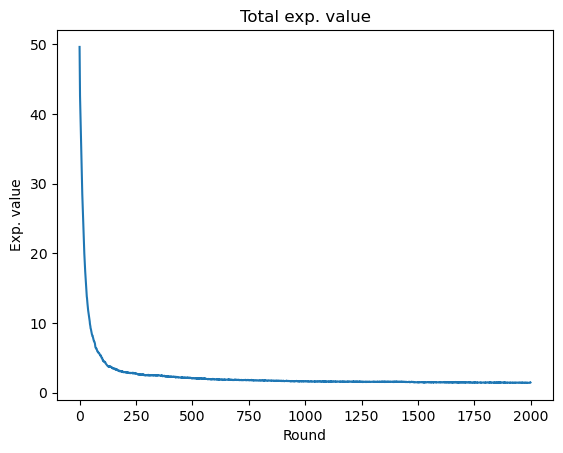
\includegraphics[width=0.45\textwidth]{chil-template-2023/images/avg_avg_exp_val.png}
    \caption{Expected value of $\ket{\psi}$ over $2000$ rounds for the semi classical approach.}
    \label{fig:avg_avg_exp_val}
\end{figure}

For this simulation we used $100$ players, $20$ elite players per round, $\pi = 0.5$, $\sigma = 0.05$ and $p = 0.5$. Using smaller mutation rates such as $\pi = 0.1$ allows for even stronger convergence to 0 and strategies which survive the longest show an almost pure $\ket{0}$ state.\\

\subsection{Collapse with Players' Average}
\label{sub: Collapse with players average}

For the next approach we keep the average to determine the players performance, for the player it is therefore still similar to simply providing real (rational) numbers. To determine $\ket{w}$ on the other hand, we use a wave function collapse, i.e. physical measurement of $\hat{N}$. We therefore have a non zero probability for any state $\ket{w}$ which we can see from small oscillations in the expected value over the course of simulations. If $|\braket{w|\hat{N}|w}|^2 \gg |\braket{0|\hat{N}|0}|^2$, only states with expected values larger than 0 make up the elite group of players and therefore increase the expected value far above the noise level for the next rounds as seen in figure \ref{fig:avg_measured_exp_val}. Eventually we can still observe an overall convergence towards $\ket{0}$ which is especially clear from looking at the state which was in the elite for the longest time over a simulation of 2000 rounds. Besides the states $\ket{0}$ and $\ket{1}$, no states have a significant weight which goes beyond the induced mutation. We show these results in figure \ref{fig:avg_measured_oldest}.

\begin{figure}[h]
    \centering
    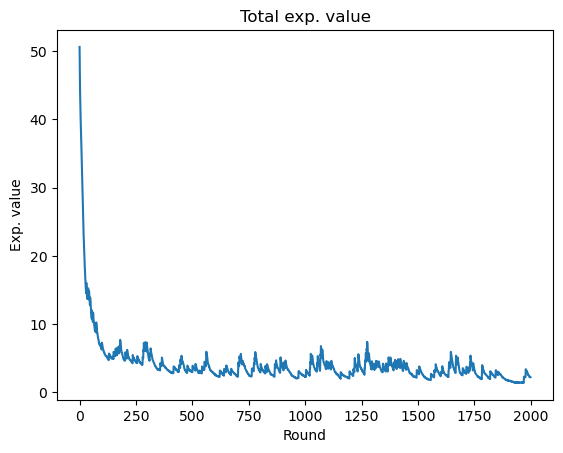
\includegraphics[width=0.45\textwidth]{chil-template-2023/images/avg_measured_exp_val.png}
    \caption{Expected value of $\ket{\psi}$ for the collapse - average game.}
    \label{fig:avg_measured_exp_val}
\end{figure}

\begin{figure}[h]
    \centering
    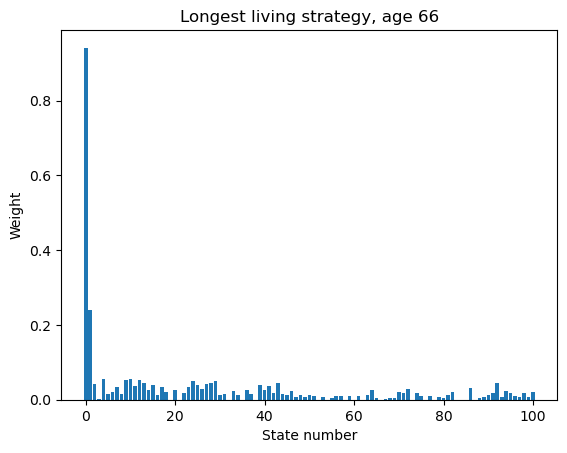
\includegraphics[width=0.45\textwidth]{chil-template-2023/Sections/avg_measured_oldest.png}
    \caption{Strategy with most rounds without an update (most rounds inside the elite).}
    \label{fig:avg_measured_oldest}
\end{figure}

For the results shown we again used $100$ players, $20$ elite players per round, $\pi = 0.5$, $\sigma = 0.05$ and $p = 0.5$. While a smaller $\pi$ leads to a decrease in the density of spikes seen in figure \ref{fig:avg_measured_exp_val}, a change to $\sigma = 0.1$ gives a non convergent game. We can therefore not find any value as a fix point. The noise is too strong for the convergence rate of the game. Interestingly this value seems to be somewhere in the region of a phase shift as for $\sigma = 0.09$ we can already see much better convergence with a lower bound of $\approx 9$.\\

\subsection{Weight of the Average: A Nonzero Equilibrium?}

With this approach we go back to using the average to determine $\ket{w}$ but we now determine the fitness from the weight each player assigned to the respective state $\ket{w}$.\\

This approach is particularly interesting as the winning players do not necessarily favor states with low averages but are only focused on the single state. This will eventually lead to a slower decay of the expected value. This is also enhanced by the mutation algorithm where the states not equal to $\ket{w}$ are uniformly distributed and only decrease in weight slowly, from the higher weight necessary on $\ket{w}$. Once the decay flattens we do not observe the expected value to reach a value around 0. Instead the expected value stays constant between 8 and 10, therefore giving $\ket{w}$ as $\ket{4}$ or $\ket{5}$. This only happens after some time by chance and shorter simulations often indicate a saturation between 10 and 12.\\

Additionally, we are able to observe large spikes of the expected value when inside a flat area. This may be caused by large mutations on higher states for multiple states in the elite, leading to a continuous boost of such features over the following rounds. An example for the course of the expected value is given in figure \ref{fig:single_avg_exp_val}.

\begin{figure}[h]
    \centering
    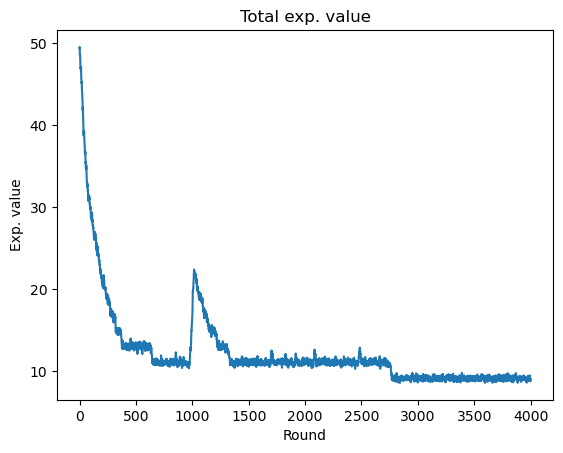
\includegraphics[width=0.45\textwidth]{chil-template-2023/images/single_avg_exp_val.png}
    \caption{Expected value of $\ket{\psi}$ for the weight of the average approach.}
    \label{fig:single_avg_exp_val}
\end{figure}

The reason for this behavior lies in the nonzero probability of higher states. Having a weight of $0.01$ on the state $\ket{100}$ increases the players expected value by $1$. As we have positive mutations on $25\%$ of the states as well as the remaining probabilities from the parents on higher states, an average of $0$ is, with the parameters as previously used in \ref{sub: The semi classical approach} and \ref{sub: Collapse with players average}, simply not possible.\\

For the exact point of convergence we were yet able to construct an exact formula but we do observe a linear scaling in $\sigma$. While the lower bound for $\sigma = 0.05$ was found to be 5, the lower bound for $\sigma = 0.01$ is determined to be 1. For such low sigma games, we also observe the establishment of dominant players which is again an effect of the mutation algorithm, although the mutations are already quite weak. Once a player finds a strategy with an almost pure 1 state, any mutation on other states leads to the a decrease in the weight of the 1 state and therefore looses against the dominant players. On the other hand, due to the rounding of $\ket{w}$, $\ket{0}$ is always a bad play if all or most players have some other non $\ket{0}$ state. We show the rounds won by each player after the saturation in figure \ref{fig:single_avg_times_won_at_1}, indicating the dominance of a few players.

\begin{figure}[ht]
    \centering
    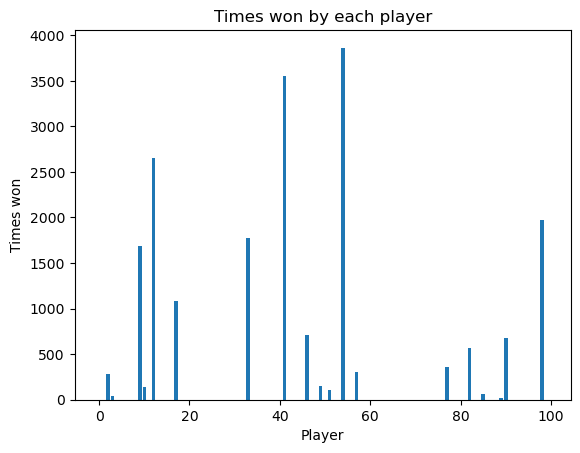
\includegraphics[width=0.45\textwidth]{chil-template-2023/images/single_avg_times_won_at_1.png}
    \caption{Times won by each player with $\sigma = 0.001$ and after boundary is reached.}
    \label{fig:single_avg_times_won_at_1}
\end{figure}

\subsection{The Projective Game}

In this approach we are using the projection of each player onto a state which is again determined by the collapse of $\ket{\psi}$ as already described in section \ref{sub: Collapse with players average}. In other words, the more likely a player is to receive the respective state upon measurement, the better its fitness. This game is quite complex for the player. For single rounds or rounds before a  clear convergence a player needs to have a good balance in their states. Distributing all probabilities evenly might not be enough to reach the elite. Putting all the weight on one card on the other hand kicks the player out of the elite for any other state. The second extreme is very much the same as betting all chips on one number at a roulette table but with a less significant reward if the state is actually found.\\

With the simulation we do find an area of uncertainty at the start of each game. With the two previous approaches we were more or less able to observe some kind of exponential decay in the expected value. With this approach on the other hand such a decay is only observed after many rounds were already played. Before that the game shows intervals of slower decay and even sections where the expected value may increase again. This behavior makes the decay already very much reliant on the seed for the random numbers which we were able to observe from decays starting after a wide range of rounds played. For our parameters this was generally still below 1000 rounds. Eventually the expected value still converges towards $\ket{0}$ were we again observe a similar behavior to the approach described in \ref{sub: Collapse with players average} with occasional spikes from non $\ket{0}$ measurements. By looking at the states $\ket{w}$ we can clearly see a phase transition from an unordered phase with many different winners to an ordered phase with only solitary non $\ket{0}$ measurements. The strategy surviving the most rounds even shows an almost pure $\ket{0}$ state with no weights above 0.1. Examples are shown in figures \ref{fig:single_measured_exp_val} - \ref{fig:single_measured_measured}.

\begin{figure}[h]
    \centering
    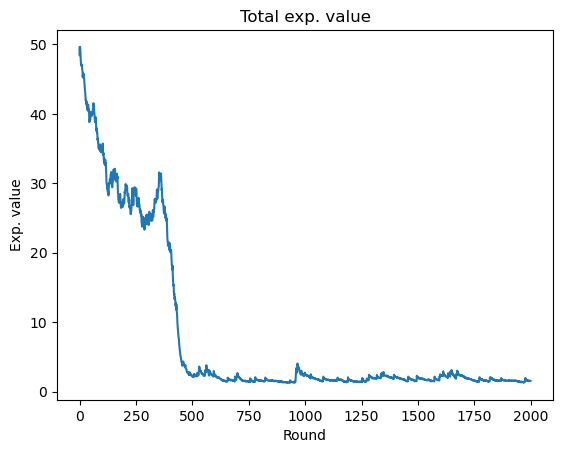
\includegraphics[width=0.45\textwidth]{chil-template-2023/images/single_measured_exp_val.png}
    \caption{expected value of $\ket{\psi}$ for the projection approach.}
    \label{fig:single_measured_exp_val}
\end{figure}

\begin{figure}[h]
    \centering
    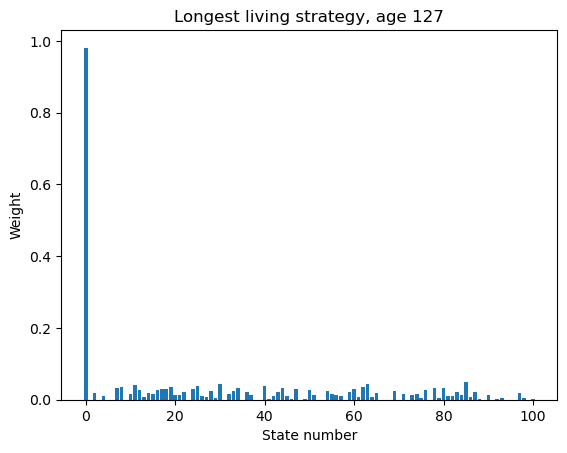
\includegraphics[width=0.45\textwidth]{chil-template-2023/images/single_measured_oldest.png}
    \caption{Longest living state for the projection approach.}
    \label{fig:single_measured_oldest}
\end{figure}

\begin{figure}[h]
    \centering
    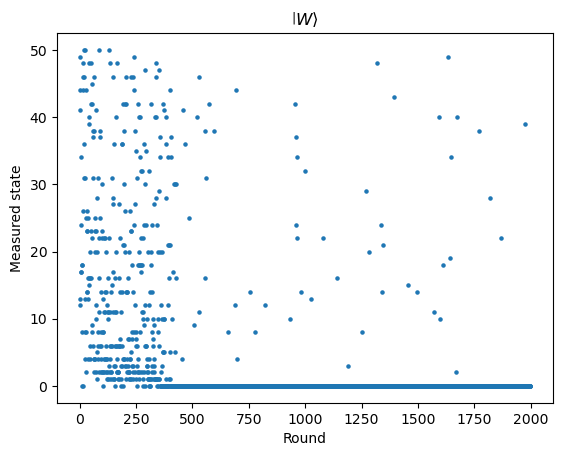
\includegraphics[width=0.45\textwidth]{chil-template-2023/images/single_measured_measured.png}
    \caption{Values of $\ket{w}$ over 2000 rounds for the projection approach.}
    \label{fig:single_measured_measured}
\end{figure}

For these results we used \texttt{np.random.seed(42)} and \texttt{np.random.seed(42)} with the first run of the simulation after setting the seed. The parameters are kept at the same values as before with $100$ players, $20$ elite players per round, $\pi = 0.5$, $\sigma = 0.05$ and $p = 0.5$. We again also try to bring up $\sigma$. Around $\sigma = 0.1$ we do not observe total chaos, as the longest living state is still dominated by $\ket{0}$ and the expected value is not distributed across all possible values. Still for $\sigma = 0.102$ we do see some form of oscillations over the course of $30.000$ rounds where we observe intervals with expected value around 15 as well as 40. At this point we do not have an explanation for this phenomena, especially why there still seems to be some order with two fix points and the system does not stabilize around $30$. What we also observe is a far more uniform distribution across all possible states in $\ket{w}$ when the expected value is around $40$ and far less measurements for states other than $\ket{0}$ when around $10$. This gives the indication that the game switches between relatively ordered and almost random states and large enough deviations from the mutation change the phase of the game. An example of this effect is shown in figure \ref{fig:single_measured_exp_val_0102}.

\begin{figure}[h]
    \centering
    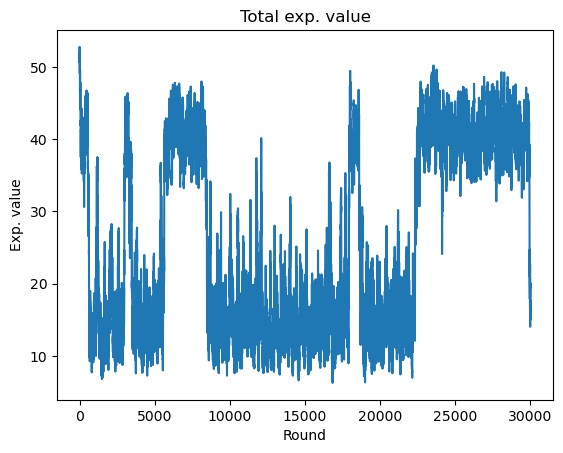
\includegraphics[width=0.45\textwidth]{chil-template-2023/images/single_measured_exp_val_0102.png}
    \caption{expected value of $\ket{\psi}$ for a simulation with on the projection game $\sigma = 0.102$.}
    \label{fig:single_measured_exp_val_0102}
\end{figure}

\subsection{Player Strategy Collapse}

Until now we have not looked at approaches where we collapsed each players strategy in order to determine the fitness score. The reason for this is simple: Using our previous approach of keeping the elite wave functions after a measurement not only seems to counter the idea of collapsing a wave function, it also leads to chaotic behavior where the expected value does not clearly converge to any point. This is regardless of determining $\ket{w}$ from the total expected value or also from a collapse of $\ket{\psi}$. Starting with almost uniform states the randomness which governs onto which state each player collapses is so large that good features (population of lower states) do not get the chance to become relevant. An example is shown if figure \ref{fig:measured_measured_exp_val}.\\

Changing the approach to setting the players strategy to its collapsed state before the next round as well as mutations does also not lead to any convergence in the expected value. Another possible change is to change the the order in the sense that we first collapse each players and then draw from the average. But even with this approach we do not see any convergence in the data again also trying out slight variations in the parameters.\\

This brings us to the conclusion that the confusion for the players is simply too large and for any described approach they are missing the incentive to develop a 'good' strategy in the sense of convergence.

\begin{figure}[h]
    \centering
    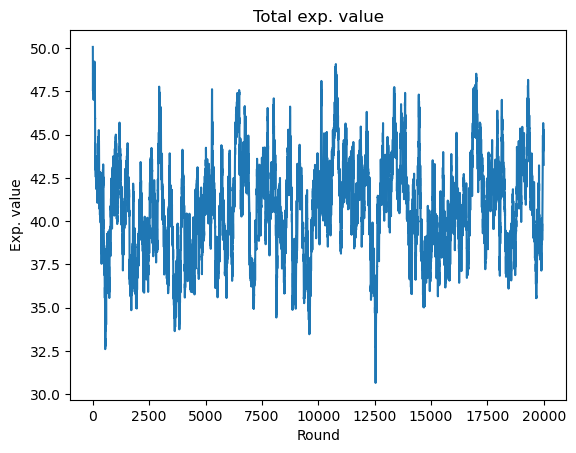
\includegraphics[width=0.46\textwidth]{chil-template-2023/images/measured_measured_exp_val.png}
    \caption{Example of a non convergent game based on wave function collapse of both $\ket{\psi}$ and all $\ket{S}$.}
    \label{fig:measured_measured_exp_val}
\end{figure}

\section{Conclusion and outlook}
With the Quantum Beauty Contest we were able to apply a formalism known from the theory of quantum mechanics onto the classical game of the Keynesian beauty contest. In particular, we looked at the case of a contractive factor $p = 1/2$ but other cases could also be easily investigated in the future.\\

With different approaches on how to determine the fitness of the strategy of a specific player we were able to observe and describe several phenomena in an evolutionary setting which are not predicted by the classical game. With phenomena such as a phase transition on the projective game approach we are able to draw connections to human behavior, in this particular example the transition from confusion to clarity on the interactions within the game. Still it is uncertain if these simulations could ever be closely reproduced by humans, considering the relatively simple mutation algorithm we used throughout the simulations. Here one could perform further investigations by limiting the amount of vector components one strategy can contain, changing the adaptation from parent strategies or limiting the precision. These might be able to closer represent a human game where people would probably only use simple fractions and not choose $101$ states for many rounds.\\

By using the principle of wave function collapse we were also able to bring some instability to the game in its equilibrium position forcing older strategies to adapt to different conditions. While strategies still show dominant $\ket{0}$ states, using the player average does not allow them to fully neglect other states. Only by using the projection operation a player is able to largely focus on this state when at the Nash equilibrium.\\

With the approach of taking the weight of the average we showed another interesting result as the game did converge but always to a state higher than $\ket{0}$. With humans it might therefore be interesting if we can reproduce such a behavior and especially to which points humans would converge. Here using smaller values for the contraction factor such as $p = 1/3$ might also be interesting to investigate in the future as this currently sets a hard boundary at $\ket{1}$ and makes a measurement of $\ket{0}$ impossible.\\

One last thing which was not considered yet by us is a variation in initial conditions. While we chose the initial states at random, leaving us with a relative uniform distribution in states, the classical game shows that most players tend to avoid numbers that are impossible to be determined as the average already on the first move. Manipulating the initial states might therefore also a a point for investigation in the future.\\
%\citep{vie2021evolutionary} % Sample Citation
%\acks{Acknowledgments}

\newpage

\bibliography{bibliography}

\appendix

\section{Supplementary Material}\label{apd:first}
The source code for the simulation can be found on \url{https://github.com/yzimmermann/QBC}.

\end{document}
